\documentclass[a4paper,11pt]{article}
\usepackage[margin=1in]{geometry}
\usepackage{graphicx}
\usepackage{setspace}
\setstretch{1.2}

\begin{document}

\title{Is Florida Getting Warmer?}
\author{}
\date{}
\maketitle

\noindent\textbf{Question.} 
Has Key West, Florida experienced an increase in temperature during the 20th century?

\vspace{0.5em}
\noindent\textbf{Data.} 
I analysed the annual mean temperature records in Key West, Florida from the years 1901 to 2000.

\vspace{0.5em}
\noindent\textbf{Method.} 
I quantified the relationship between year and annual mean temperature using the Pearson correlation coefficient. 
To test whether the observed trend could have arisen by chance, a permutation test was performed with 10{,}000 randomisations. 
In each permutation, temperature values were randomly reassigned to years to generate a null distribution of correlation coefficients. 
The p-value was calculated as the proportion of random correlations greater than or equal to the observed correlation.

\vspace{0.5em}
\noindent\textbf{Results.} 
The observed correlation between year and temperature was $r = 0.53$, showing a moderate positive relationship. 
The permutation test produced an approximate one-sided p-value of $p \approx 0.001$, meaning that fewer than 0.1\% of randomised datasets produced a correlation as strong as the observed one.

\begin{figure}[h!]
    \centering
    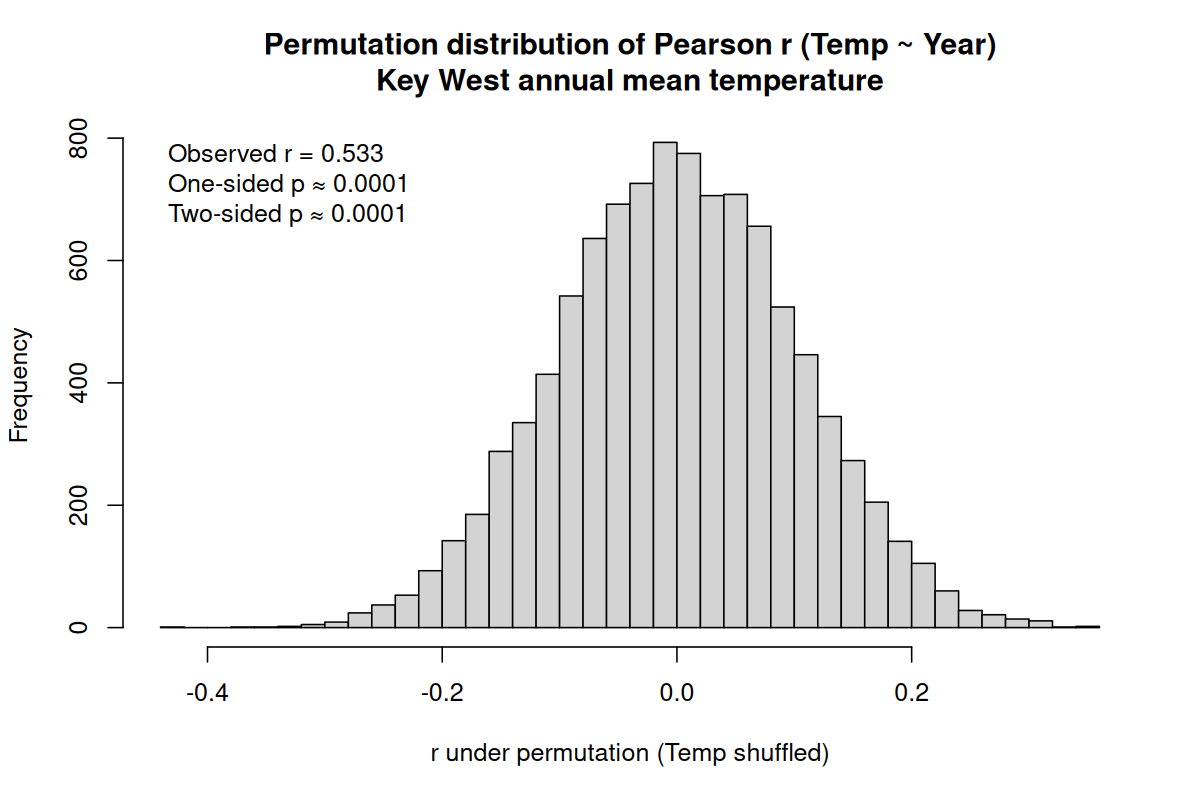
\includegraphics[width=0.85\textwidth]{../results/perm_hist.png}
    \caption{Permutation distribution of Pearson correlation coefficients between Year and Temperature in Key West, Florida. 
    The vertical red line shows the observed correlation, which lies far to the right of the null distribution.}
\end{figure}

\vspace{0.5em}
\noindent\textbf{Interpretation.} 
The analysis showed that strong evidence that mean annual temperatures in Key West increased significantly over the 20th century (from the year of 1901 to 2000). 
The positive correlation (r = 0.53) and extremely low p-value indicate a consistent warming trend that is unlikely to have occurred by random chance. 
In conclusion, Key West, Florida has indeed become warmer during the 20th century.

\end{document}
